\chapter{ روش پیشنهادی }
\section{مقدمه}

همان‌طور که در فصل‌ گذشته شرح داده شد، شناسایی بی‌درنگ چهره در محیط بدون محدودیت و با دقت بالا با چالش‌های بسیاری همراه است. همچنین دقت بالا و زمان پردازش سریع باهم در تقابل هستند. علاوه بر این‌ها، فرض ‌کمبود داده آموزشی نیز چالش بزرگی محسوب می‌شود. بنابراین در این فصل تلاش می‌کنیم تا روشی برای تشخیص دقیق‌تر و بی‌درنگ چهره توسط شبکه عصبی عمیق در تصاویر بدون محدودیت پیشنهاد دهیم. در ابتدا مرحله پيش پردازش شرح داده مي‌شود. در قسمت بعد، رويكرد استفاده شده مبتني بر شبكه‌هاي پيچشي به منظور استخراج ویژگی از تصاوير چهره شرح داده خواهد شد. نمای کلی روش ارائه شده در شكل \ref{image4-1} خلاصه شده است كه در ادامه هر يک تشريح خواهد شد. 
\begin{figure}[h]
\centering
  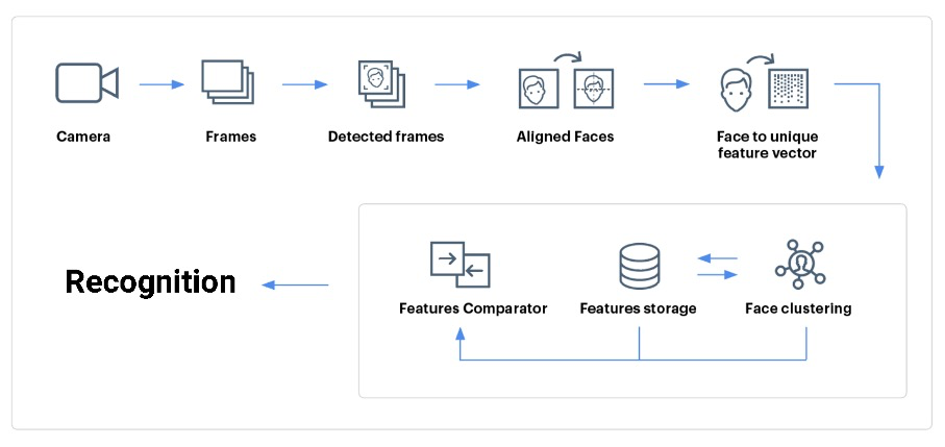
\includegraphics[width=1.0\textwidth]{image1-1}
  \caption{نمای کلی از روش پیشنهادی \cite{ref1}.}
  \label{image4-1}
\end{figure}

\section{پیش پردازش}
بيشتر الگوريتم‌ها‌ي شناسایی چهره نياز به اعمال پيش‌پردازش‌هايي بر روي تصوير ورودي دارند. در این روش، پیش‌پردازش شامل همسان سازی بافت‌نگار به منظور افزایش تباین، یافتن چهره و تراز کردن تصویر می‌باشد. در ادامه به شرح مراحل پیش‌پردازش می‌پردازیم.
\subsection{همسان سازی بافت‌نگار}
یکی از روش‌های بهبود تصویر، افزایش تباین تصویر است. یکی از روش‌های افزایش تباین تصویر، تکنیک یکنواخت سازی بافت‌نگار است. بطوریکه مقادیر پیکسل‌های تصویر را طوری تغییر می‌دهد تا کل بازه ممکن را تسخیر کند و ایده اساسی آن. نگاشت مقادیر شدت سطوح روشنایی از طریق یک تابع توزیع انتقال است. این عمل باعث افزایش تباین تصویر  می‌شود که به معنای بهبود کیفیت تصویر و افزایش دقت پردازش های بعدی است. نمونه ای از این روش را از مقاله \cite{s18092995} در شکل \ref{image4-2}  مشاهده می‌نمایید.
\begin{figure}[h]
\centering
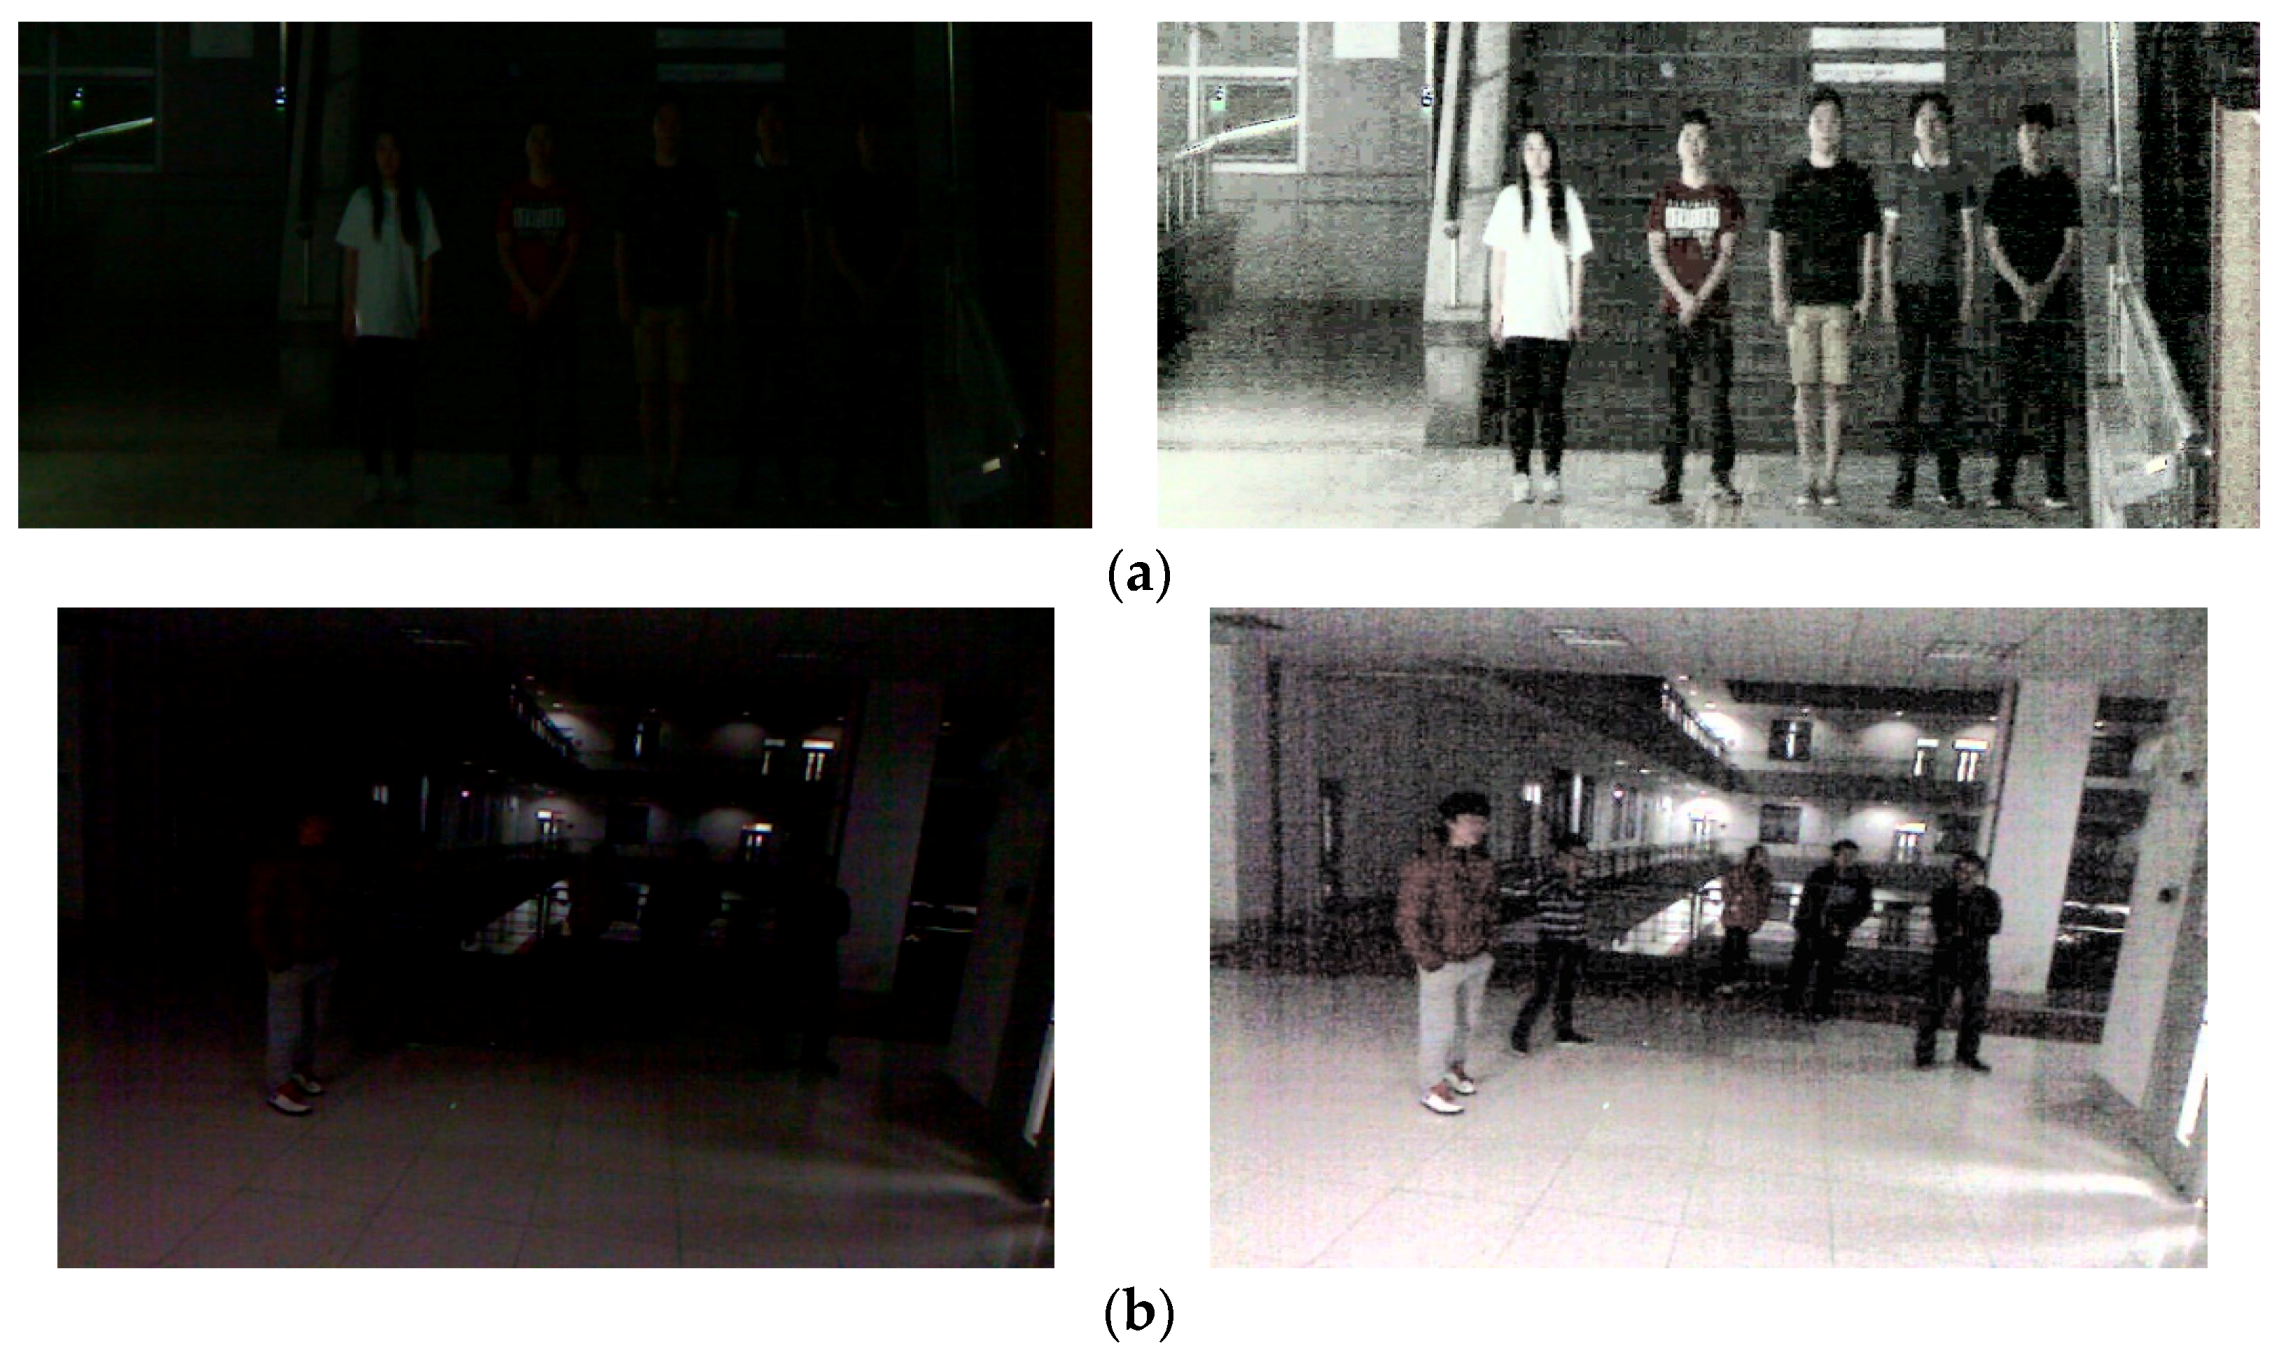
\includegraphics[scale=1]{image4-2}
\caption{نتیجه اعمال یکسان سازی بافت‌نگار بر روی یک تصویر تاریک. تصاویر ورودی در سمت چپ و خروجی در سمت راست می‌باشند \cite{s18092995}.}
\label{image4-2}
\end{figure}

\subsection{یافتن چهره}
يكي ديگر از مراحل معمول پيش پردازش كه در طي فرآيند شناسایی چهره انجام مي‌شود، مکان یابی و یافتن چهره در تصاوير مي‌باشد. برای این منظور از یک روش مبتنی بر شبکه عصبی پیچشی که توسط \lr{Deng} و همکاران \cite{deng2019retinaface} در سال ۲۰۱۹معرفی شده است استفاده می‌کنیم. در این روش برای آموزش شبکه پیچشی از یک تابع ضرر مبتنی بر یادگیری چندکاره \LTRfootnote{Multi Task Learning} استفاده شده است که به صورت زیر می‌باشد.
\begin{equation}\label{eq3-2}
L = L_{cls} + L_{box} + L_{pts} + L_{pixel}  
\end{equation}
\noindent
که در آن $L_{cls}$ تابع ضرر مربوط به یافتن یا عدم یافتن چهره می‌باشد. $L_{box}$ تابع ضرر مربوط به مکان چهره می‌باشد. همچنین $L_{pts}$ تابع ضرر مربوط به یافتن نقاط ویژه روی اجزای چهره می‌باشد، و $L_{pixel}$ تابع ضرر مربوط به یافتن یک مدل سه بعدی مبتنی بر مش از روی چهره می‌باشد. استفاده از تابع ضرر مبتنی بر یادگیری چند کاره، کمک می نماید تا فضای مسئله محدود تر شود و الگوریتم بهینه سازی مورد نظر زودتر به سمت نقطه بهینه همگرا شود. ما برای رسیدن به خروجی بی درنگ، این روش را بر روی معماری \lr{MobileNetV3} پیاده سازی کرده و آموزش دادیم. نمونه ای از خروجی این روش را در شکل \ref{image4-3} مشاهده می‌کنید. 
\begin{figure}[h]
\centering
  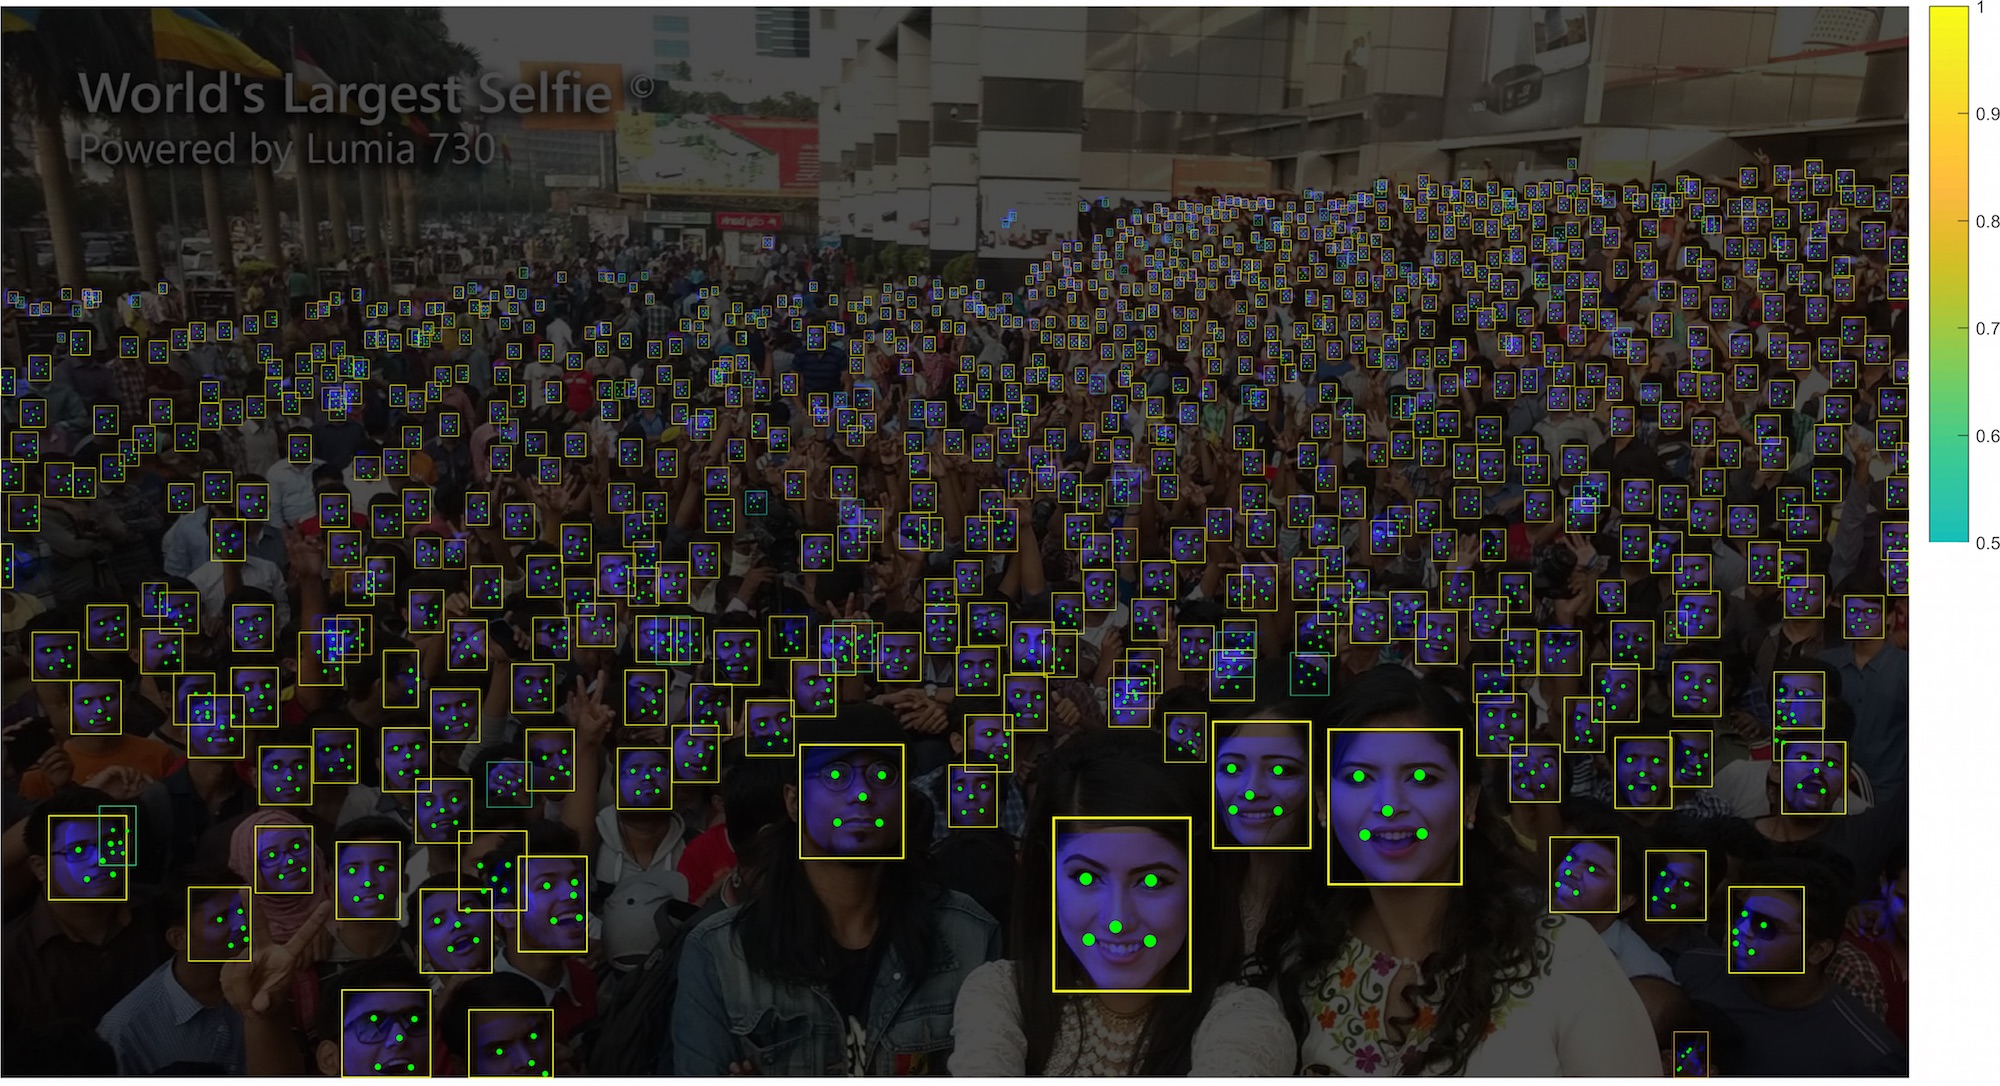
\includegraphics[width=1.0\textwidth]{image4-3}
  \caption{نمونه از خروجی الگوریتم یافتن چهره retina \cite{deng2019retinaface}.}
  \label{image4-3}
\end{figure}

\subsection{تراز کردن تصویر}
در ادامه روند پیش‌پردازش، نوبت به تراز کردن تصویر چهره \LTRfootnote{Face Alignment} می‌رسد. پس از یافتن چهره، به تصویر ورودی مناسب شبکه نزدیک تر می‌شویم، اما پس از تراز کردن تصویر جهت آموزش شبکه، بهبود دقت نهایی مشهود است.  بدین منظور با استفاده از یک تبدیل غیرخطی، تصویر چهره را به گونه ای می‌چرخانیم که چشم،ها در راستای خط افقی قرار بگیرند. روش‌های کلی برای تشخیص چهره از زاویه‌ی روبه‌رو به خوبی عمل می‌کنند اما مقاومت این روش‌ها در مقابل تغییرات زاویه مناسب نیست، به این علت که ویژگی‌های ظاهری با تغییرات زاویه بسیار تغییر پذیر هستند. با تراز کردن تصویر چهره پیش از اعمال طبقه‌بند می‌توان این مشکل را بهبود داد. در طول ‌تراز کردن تصویر، نقاط خاصی از تصویر (مانند نقطه‌ وسط دو چشم و نقاط دو طرف دهان) در نظر گرفته می‌شود و به مختصات مشخصی منتقل می‌شوند. برای این منظور از ۵ نقطه ویژه استخراج شده در مرحله یافتن چهره توسط الگوریتم retina استفاده می‌کنیم. نتیجه اعمال این فرآیند را در شکل \ref{image4-4} مشاهده می‌کنید. در نهایت تصاویر چهره با اندازه ۱۱۲ * ۱۱۲ پیکسل ذخیره می‌گردند تا در مرحله آموزش شبکه، مورد استفاده قرار گیرند.
\begin{figure}[h]
\centering
  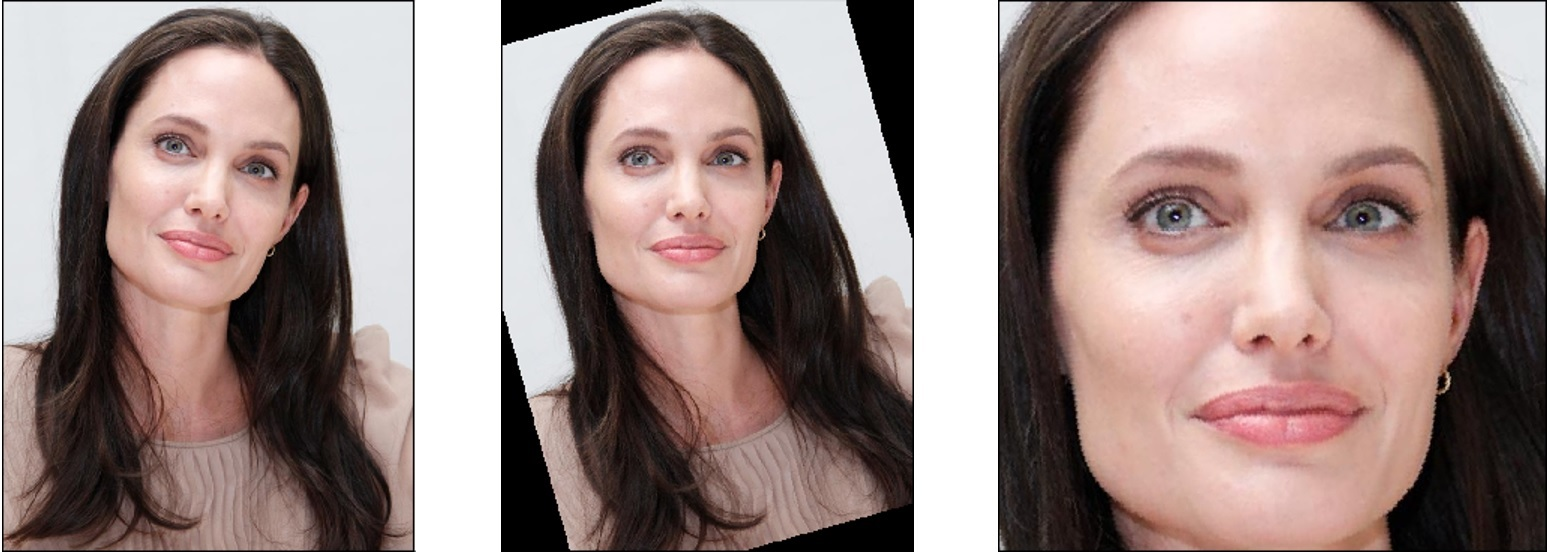
\includegraphics[width=1.0\textwidth]{image4-4}
  \caption{به منظور افزایش دقت شبکه، پس از یافتن چهره باید آن را تراز کرد \cite{}.}
  \label{image4-4}
\end{figure}

\section{دسته بندی}
روش پیشنهادی برای تشخیص بی‌درنگ چهره در محیط های بدون محدودیت، یک الگوریتم مبتنی بر شبکه های پیچشی می‌باشد. این فرایند را می توان به صورت یک مسئله بهینه سازی فرموله کرد که در ادامه به بخش های مختلف آن می پردازیم.

\subsection{مدل پيشنهادي پايه}
در این بخش ابتدا باید معماری مناسب شبکه پایه برای مسئله را به دست آوریم. با بررسی شبکه‌های متداول و مقایسه دقت و زمان پاسخگویی آن‌ها به کمک یادگیری انتقال، به این نتیجه می‌رسیم که شبکه \lr{MobileNetV3} دارای چگالی دقت بالاتری در مقایسه با شبکه های دیگر می‌باشد و نسبت دقت دسته بندی به تعداد پارامترهای شبکه در آن‌ بیشتر می‌باشد. بنابرین می‌توان سرعت اجرای مناسب و همچنین دقت مناسب را از این شبکه‌ انتظار داشت. از نتایج در می‌یابیم که بهترین معماری شبکه برای مسئله ما معماری \lr{MobileNetV3} است. نتایج آزمایش در جدول \ref{table4-1} آمده است. آزمایش‌هایی بر روی معماری‌های مطرح دیگر نیز انجام شد که به علت ضعیف بودن نتایج یا بالا بودن زمان پاسخ دهی در جدول درج نشده اند.
\begin{table}[ht]
\label{table:5-1}
\begin{center}
\caption{مقایسه و ‌ارزیابی برخی از معماری شبکه های رایج در زمینه بینایی ماشین}
\resizebox{\textwidth}{!}
{
\begin{tabular}{|c|c|c|c|}
\hline 
نام شبکه & تعداد پارامترها & دقت بر روی مجموعه داده LFW
\\
\hline 
MobileNetV2 & 3.53M & 93.50
 \\
\hline
MobileNetV3 & 2.5M & 95.8 	 
\\
\hline
SqueezeNet & 1.25M & 89.2
\\
\hline 
NASNetMobile & 5.32M & 90.60
\\
\hline
EfficientNetB0 & 5.3M & 85.50
\\
\hline
\end{tabular}
}
\end{center} 
\end{table} 
\noindent
تشخيص چهره به دليل وجود پيكسل‌هاي مشابه از نظر شدت روشنايي در تصویر بسيار چالش برانگيز بوده است. از آنجا كه عمليات كانولوشن به پنجره محلي از شدت روشنايي پیکسل‌هاي تصوير هدايت مي‌شود، بنابراين، اين امكان وجود دارد كه ويژگي‌هاي مربوط به پیكسل‌های تصاویر داراي برچسب يكسان، تفاوت‌هايی داشته باشند و يا ويژگي‌های مربوط به پیكسل‌های تصاویر داراي برچسب متفاوت، يكسان باشند. اين اختلالات باعث کاهش جداپذیری بردارهای ویژگی خروجی مي‌شوند. براي حل اين مشكل، از اطلاعات كلی تصاوير به وسيله لايه‌های توجه استفاده می‌کنیم. لايه توجه استفاده شده در اين پژوهش، شامل لایه توجه وابسته به كانال و لایه توجه وابسته به موقعيت مي‌باشد. معماری شبکه پیشنهادی در شکل \ref{image4-5} آمده است.

\begin{figure}[h]
\centering
  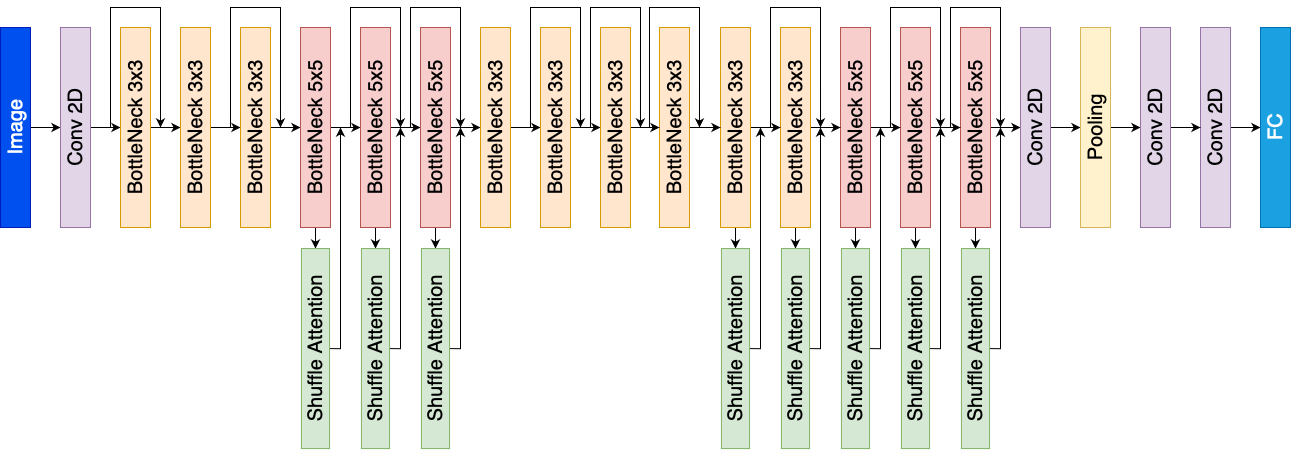
\includegraphics[width=1.0\textwidth]{image4-5}
  \caption{مدل پايه مبتني بر لايه‌هاي كانولوشن و لايه توجه.}
  \label{image4-5}
\end{figure}

\noindent
در این معماری مسير استخراج ويژگي از ۴ لايه كانولوشن، ۱ لایه رای گیری، ۱۵ لايه تنگنا \LTRfootnote{Bottleneck}  و ۸ ماژول توجه \LTRfootnote{Attention} تشکیل شده است، كه در ادامه توضيح داده خواهد شد، تصوير ورودي به بخش استخراج ويژگي داده مي‌شود و مدل در اين مسير به طور خودكار يك سلسله مراتب ويژگي را از تصاوير ورودي آموزش خواهد ديد و در نهايت اين ويژگي‌هاي استخراج شده به عنوان ورودي دسته بند مورد استفاده قرار مي‌گيرد.

\subsubsection{لايه كانولوشن}
۴ لایه کانولوشن دو بعدی همراه با گام یک یا دو استفاده شده است. در اولین لایه کانولوشن‌ اندازه پنجره فیلترها $3 \times 3$ و در لایه های کانولوشن بعدی اندازه پنجره فیلتر ها $1 \times 1$ می‌باشد. دلیل انتخاب سایز کوچک پنجره فیلترها کاهش پیچیدگی محاسباتی و همچنین عملکرد خوب آن‌ها در استخراج ویژگی می‌باشد. چگونگی عملکرد یک لایه کانولوشن از رابطه \ref{eq4-1} بدست می‌آید.
\begin{equation}	
x_j^{(l)} =\sum_{i=0}^{c} w_{c_{ij}}^{(l)}\ast x_i^{(l-1) }+ b_j^{(l)} 
\label{eq4-1}
\end{equation}

\noindent
که در آن $l$ نشان دهنده شماره لایه کانولوشن، $b$ و $w$ پارامترهای مدل، $x$ خروجی هر لایه $j\in[1,n]$ بیانگر شماره فیلتر موجود درلایه $l$ و همچنین $n$ بیانگر تعداد کل فیلترها در لایه $l$ و $\ast$ نشان دهنده عملگر کانولوشن می‌باشد.

\subsubsection{لایه تنگنا و واحد باقیمانده}
به عنوان مثال به جای پردازش یک نگاشت ویژگی عظیم با 256 عمق، ابتدا همه این اطلاعات را در نگاشت‌های ویژگی 64 بعدی فشرده می‌کنیم. زمانی که این فشردگی انجام شد، از کانولوشن 3×3 استفاده می‌کنیم که وقتی روی 64 نگاشت ویژگی به جای 256 نگاشت اعمال شود، بسیار سریع‌تر است و چنین پردازشی می‌تواند همان نتایج یا نتایج بهتری نسبت به پشته‌های معمولی 3×3 ارائه کند. در نهایت با استفاده از 1×1 مجدداً به نگاشت اصلی 256 خود بازمی‌گردیم.

\noindent
از سوی دیگر شبکه‌های عمیق با واحدهای باقیمانده\LTRfootnote{Deep Residual Network}  بر روی پایگاه داده‌های مختلف مانند \lr{ImageNet}  و COCO، دقت و همگرایی خوبی را از خود نشان داده‌اند. با استفاده از مسیرهای پرش\LTRfootnote{Shortcut Pathway}، واحدهای باقیمانده می‌توانند به سیگنال‌ها اجازه دهند که مستقیماً از یک بلوک به بلوک‌های دیگر منتقل شوند. به طور کلی، واحدهای باقیمانده را می‌توان به صورت رابطه \ref{eq4-2} بیان کرد.
\begin{equation}
x_{l+1}=x_l+R(x_l ,w_l)
\label{eq4-2}
\end{equation}

\noindent
در اینجا $R$ نشان دهنده تابع واحد باقیمانده است، $x_l$ ویژگی ورودی به واحد باقیمانده $l$ام و $W_l$ مجموعه‌ای از پارامترهای مربوط به واحد باقیمانده $l$ام می‌باشد. ایده اصلی شبکه‌های باقیمانده، عمیق‌تر کردن یک شبکه به منظور افزایش دقت شبکه مورد نظر می‌باشد. بنابراین با این عملیات در واقع به شبکه اجازه داده می‌شود که در صورت نیاز، ویژگی‌های لایه قبل بدون تغییر و به صورت مستقیم به لایه بعد منتقل شود. در شکل \ref{image4-6} لایه تنگنا با واحد باقیمانده طراحی شده در این مدل به نمایش گذاشته شده است.

\begin{figure}[h]
\centering
  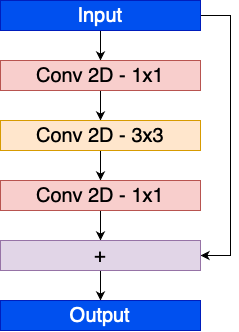
\includegraphics[width=0.25\textwidth]{image4-6}
  \caption{یک لایه تنگنا با واحد باقیمانده که با استفاده از کانولوشن های 1×1 اقدام به کاهش ابعاد نگاشت ویژگی می‌کند.‌.}
  \label{image4-6}
\end{figure}

\subsubsection{واحد توجه}
لایه توجه استفاده شده در این پژوهش یک واحد توجه SA \LTRfootnote{Shuffle Attention} است که در مقاله \cite{yang2021sanet} معرفی شده است. این لایه ابتدا ابعاد کانال را به چندین ویژگی فرعی قبل از پردازش موازی آنها تقسیم می‌کند. سپس، برای هر زیر ویژگی از یک واحد Shuffle برای به تصویر کشیدن وابستگی های ویژگی در هر دو بعد مکانی و کانال استفاده می‌کند. پس از آن ، همه زیر ویژگی ها جمع می شوند و یک عملگر تغییر کانال برای امکان برقراری ارتباط اطلاعاتی بین ویژگی های فرعی مختلف به کار گرفته می شود. معماری این ماژول در شکل \ref{image2-32} آمده است. این لایه شامل دو بخش اصلی وابسته به کانال\LTRfootnote{Channel Attention Module}  و وابسته به موقعیت \LTRfootnote{Spacial Attention Module}  می‌باشد. 

\begin{figure}[h]
\centering
  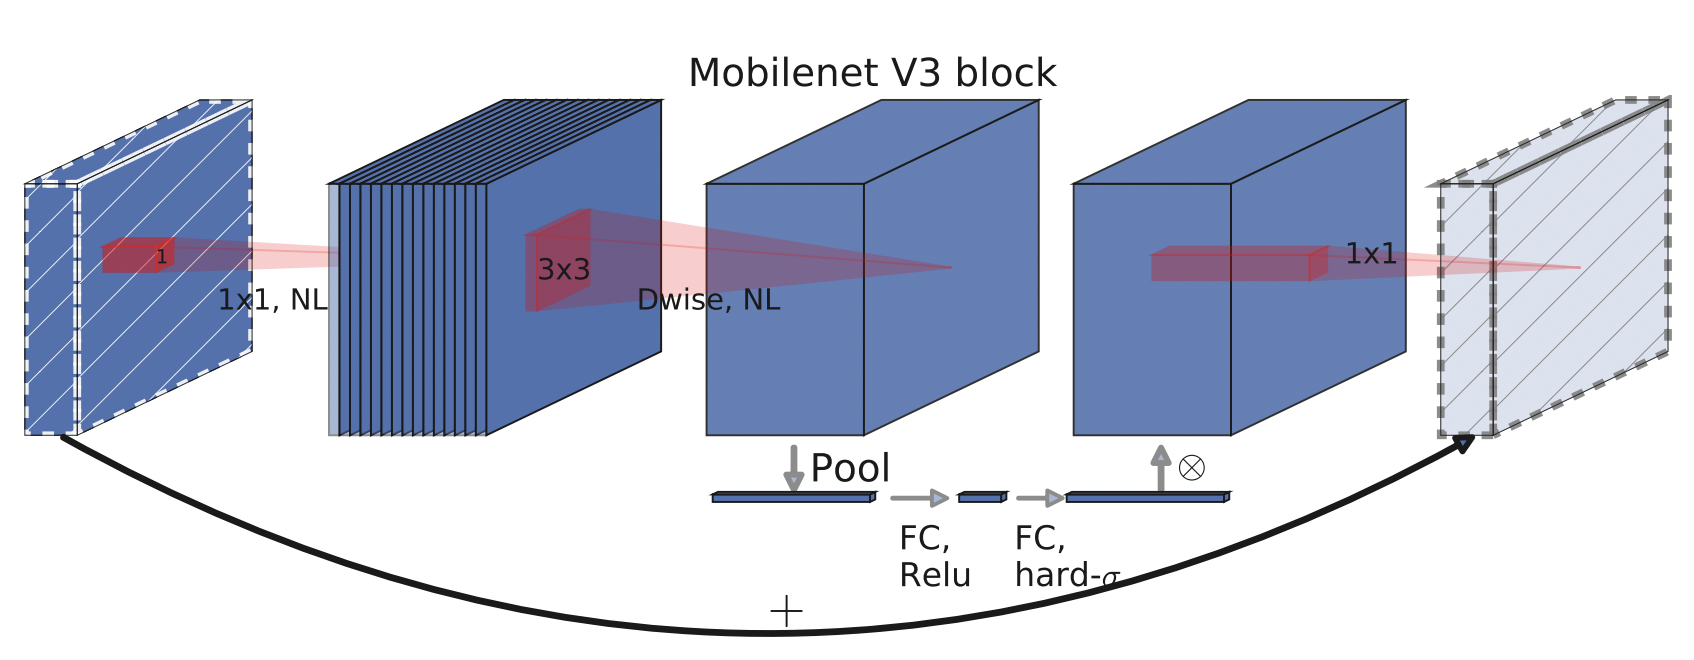
\includegraphics[width=1\textwidth]{image2-32}
  \caption{
  معماری ماژول Shuffle Attention
   \cite{yang2021sanet}.}
  \label{image2-32}
\end{figure}

\noindent
یک نقشه ویژگی \LTRfootnote{feature map} به نام $X$ با ابعاد $C \times H \times W$ که در آن $C$ و $H$ و $W$ به ترتیب عمق کانال، ارتفاع و عرض هستند، به عنوان ورودی واحد توجه در نظر گرفته می‌شود. ابتدا $X$ به $G$ گروه در طول کانال تقسیم می‌شود. رابطه \ref{eq4-3} این موضوع را نشان می‌دهد. سپس هر $X_k$ در طول کانال به دو نیم تقسیم شده و $X_{k1}$ و $X_{k2}$ را تشکیل می‌دهند. یکی از این دو زیر نقشه ویژگی  \LTRfootnote{sub feature map} برای توجه وابسته به کانال و دیگری برای توجه وابسته به موقعیت مورد استفاده قرار می‌گیرد. این عملیات توجه به مفهوم چه چیزی؟ و کجا؟ معنا می‌بخشد. 

\begin{equation}
X = [X_1, ..., X_G], X_k \in \mathbb{R}^{C/G \times H \times W}
\label{eq4-3}
\end{equation}

\noindent
برای اتصال صحیح ماژول واحد توجه به معماری \lr{MobileNetV3} مقدار $G$ را برابر ۴ در نظر گرفتیم.

\textbf{توجه  وابسته به کانال}
با بهره‌گیری از وابستگی‌های بین کانال‌ها، می‌توان بر ویژگی‌های وابسته، تأکید کرده و استخراج ویژگی‌های معانی خاص را بهبود بخشید. بنابراین در این پژوهش یک ماژول توجه وابسته به کانال ایجاد شده تا به طور واضح وابستگی بین کانال‌ها را مدل کند. ابتدا نقشه ویژگی $X_{k1}$ که از مرحله قبل بدست آمده است، توسط یک لایه پولینگ میانگین گیر سراسری \LTRfootnote{Global Averaging Pooling} به یک نقشه ویژگی $s$ با ابعاد $C/2G \times 1 \times 1$ تبدیل می‌شود. رابطه \ref{eq4-4} نشان دهنده چگونگی ایجاد بردار نقشه توجه وابسته به کانال می‌باشد. 

\begin{equation}
s = \frac{1}{H \times W}\sum_{i=1}^{H} \sum_{j=1}^{W} X_{k1} (i, j)
\label{eq4-4}
\end{equation}

\noindent
با انجام این عملیات، اطلاعات مکانی کلی برای هر کانال به صورت جداگانه محاسبه می‌شود و در $s$ قرار می‌گیرد. سپس خروجی لایه توجه وابسته به کانال مطابق رابطه \ref{eq4-5} بدست ‌می‌آید. 

\begin{equation}
X^{\prime}_{k1} = \sigma(W_1 s + b_1) . X_{k1}
\label{eq4-5}
\end{equation}

\noindent
که در آن $W_1\in R^{C/2G \times 1 \times 1} $  و  $b_1\in R^{C/2G \times 1 \times 1} $ به ترتیب نشان دهنده وزن و بایاس می‌باشند. ‌‌‌سپس نقشه توجه وابسته به کانال بدست آمده در نقشه ویژگی‌های ورودی ضرب شده و خروجی حاصل را ارائه می‌دهد.

\textbf{توجه وابسته به موقعیت}
وجود ویژگی‌های متمایز برای درک تصویر ورودی ضرروی می‌باشد، که این ویژگی‌ها می‌تواند در بازه بزرگی از تنوع قرار بگیرند. به منظور مدل سازی روابط مبتنی  بر روی ویژگی‌های محلی، ماژول توجه وابسته به موقعیت استفاده می‌شود. ابتدا ورودی $X_{k2}$ توسط یک عملگر GN \LTRfootnote{Group Norm} نرمال سازی می‌شود و خروجی این مرحله طبق رابطه \ref{eq4-6} بدست می‌آید.

\begin{equation}
X^{\prime}_{k2} = \sigma(W_2 GN(X_{k2}) + b_2) . X_{k2}
\label{eq4-6}
\end{equation}

\noindent
که در آن $W_2\in R^{C/2G \times 1 \times 1} $  و  $b_2\in R^{C/2G \times 1 \times 1} $ به ترتیب نشان دهنده وزن و بایاس می‌باشند. ‌‌‌سپس نقشه توجه وابسته به کانال بدست آمده در نقشه ویژگی‌های ورودی ضرب شده و خروجی حاصل را ارائه می‌دهد. در نهایت نقشه ویژگی های  $X^{\prime}_{k1}$ و $X^{\prime}_{k2}$ در کنار هم قرار گرفته و نقشه ویژگی 
$X^{\prime}_{k} \in \mathbb{R}^{C/G \times H \times W}$
بدست می‌آید. 

\textbf{تجمع}
پس از مراحل بالا، تمام زیر ویژگی‌های $X_k$ جمع می شوند و سرانجام یک عملگر مخلوط کننده کانال \LTRfootnote{channel shuffle} را برای ادغام اطلاعات گروه‌ها در طول بعد کانال به کار می‌بریم. خروجی نهایی واحد توجه به همان اندازه $X$ است که یکپارچه سازی SA با معماری های مدرن را آسان می‌‌کند ٖ\cite{yang2021sanet}.

\subsection{تابع ضرر}
یکی از چالش های اصلی در یادگیری ویژگی ها با استفاده از شبکه های عصبی عمیق پیوسته \lr{(DCNN)} برای شناسایی چهره در مقیاس بزرگ، طراحی تابع ضرر مناسب است که قدرت تفکیک را افزایش دهد. از آن‌جایی که ‌شبکه \lr{MobileNetV3} معماری بسیار سبک تری نسبت به معماری‌های شناخته شده دیگر که در فصل ۲ معرفی شدند، دارد؛ بنابراین استخراج ویژگی‌ها از چهره و دسته بندی تصاویر چهره با دقت بالا برای این شبکه بسیار دشوار است. همچنین در مواردی شباهت چهره افراد به یکدیگر ‌کار را از آن‌چه هست سخت‌تر خواهد کرد. تابع ضرر ArcFace \cite{deng2019arcface} کمک می‌کند ویژگی‌های استخراج شده که متعلق به دو دسته متفاوت هستند، فاصله بیشتری از هم داشته باشند و در مقابل ویژگی های استخراج شده برای دو تصویر از چهره یک فرد یکسان، فاصله کمتری از هم داشته باشند؛ این تابع ضرر که می‌توان آن را به راحتی با هزینه‌های محاسباتی ناچیز پیاده سازی کرد، به کاهش مشکلات ذکر شده کمک می‌نماید. 
\noindent
رابطه ریاضی \lr{softmax} معروف ترین تابع ضرر طبقه بندی که به طور گسترده استفاده می‌شود، به صورت رابطه \ref{eq4-7} است.

\begin{equation}
L= - \frac{1}{N} \sum_{i=1}^{N} log \frac{e^{{W_{y_i}^T} x_i + b_{y_i}}}{\sum_{j=1}^{n} e^{{W_j^T} x_i + b_j}} 
\label{eq4-7}
\end{equation}

\noindent
که در آن \lr{xi} نشان دهنده ویژگی عمیق نمونه \lr{i} ازدسته \lr{y} است. تعداد ابعاد ویژگی استخراج شده را 512 در نظر گرفتیم. \lr{Wj} ستون \lr{j}  ام از وزن \lr{W} می‌باشد و \lr{bj} بایاس است. مقدار \lr{N}اندازه دسته و \lr{n} تعداد دسته‌ها است. از آنجا که تابع $softmax$ ذات زاویه ای و قطبی دارد، بنابرین می‌توان آن را به صورت رابطه \ref{eq4-8} بازنویسی کرد:

\begin{equation}
L = - \frac{1}{N} \sum_{i=1}^{N} log \frac{e^{\left\|W_{y_i}\right\| \left\|x_i\right\| cos(\theta_{y_i})}}{\sum_{j=1}^{n} e^{\left\|W_j\right\| \left\|x_i\right\| cos(\theta_j)}}
\label{eq4-8}
\end{equation}

\noindent 
در این تابع ابتدا بردار ویژگی ‌$x$ که خروجی آخرین لایه شبکه می‌باشد، نرمال می‌شود. همچنین وزن‌های $W$ مربوط به آخرین لایه شبکه نیز نرمال‌سازی می‌شوند. بنابراین می‌توان برای سادگی اندازه $\left\|x_i\right\|$ را برابر مقدار ثابت $s$ و اندازه $\left\|W_j\right\|$ را برابر صفر در نظر گرفت. بنابرین ویژگی‌های استخراج شده در یک ابر کره با شعاع s توزیع می‌شوند.همچنین مقدار $b_j$ را برابر صفر در نظر می‌گیریم. تابع نهایی به صورت رابطه \ref{eq4-9} نوشته می‌شود.

\begin{equation}
L = - \frac{1}{N} \sum_{i=1}^{N} log \frac{e^{s(cos(\theta_{y_i}+m))}}{\sum_{j=1}^{n} e^{s(cos(\theta_j + m))}}
\label{eq4-9}
\end{equation}

\noindent 
حاصل ضرب وزن‌‌ها در ویژگی های استخراج شده محاسبه می‌گردد، که برابر $cos(\theta_j)$ می‌شود‌‌. سپس $arccos$ آن محاسبه شده که مقدار $\theta_j$ را به ما می‌دهد. سپس برای افزایش حاشیه بین \lr{xi} و \lr{Wj} یک مقدار حاشیه زاویه ای $m$ به زاویه هدف اضافه می‌کنیم‌ تا به طور همزمان فشرده سازی درون کلاسی و اختلاف بین کلاسی را افزایش دهیم.، در انتها دوباره $cos(\theta_j)$ محاسبه شده و در ثابت $s$ ضرب می‌شود.  مراحل بعدی دقیقاً مانند \lr{softmax} هستند. در این روش بنا به پیشنهاد مقاله \cite{deng2019arcface} مقدار $m=0.5$ و مقدار $s=64$ در نظر گرفته شده است. مزایای این روش پیشنهادی را می‌توان به شرح زیر خلاصه کرد:

\begin{itemize}
 \item
در مجموعه داده های تصویر و فیلم در مقیاس بزرگ‌، به عملکرد مناسبی دست می‌یابد.
 \item
فقط به چندین خط کد نیاز دارد و اجرای آن در چارچوب های یادگیری عمیق مبتنی بر \lr{Pytorch} و \lr{Tensorflow} آسان است. برای داشتن عملکرد پایدار نیازی به ترکیب با سایر توابع ضرر ندارد و به راحتی همگرا می‌شود.
 \item
هنگام آموزش فقط پیچیدگی محاسباتی ناچیز را اضافه می کند. پردازنده های گرافیکی کنونی می توانند به راحتی از هزاران دسته مختلف برای آموزش پشتیبانی کنند و مدل به راحتی می تواند هویت های بیشتری را پشتیبانی کند.
\end{itemize} 

همانطور که در شکل \ref{image4-7} نشان داده شده است، \lr{softmax} ویژگی‌های تقریباً قابل تفکیکی ایجاد می‌کند اما در مرزهای تصمیم گیری ابهام قابل توجهی به وجود می‌آید، در حالی که تابع ضرر ArcFace می تواند فاصله بیشتری را بین دسته‌های نزدیک اعمال کند.
\begin{figure}[h]
\centering
  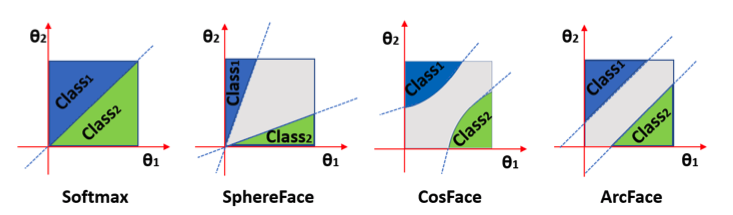
\includegraphics[width=1\textwidth]{image4-7}
  \caption{تابع ضرر ArcFace در مقایسه با توابع ضرر مشهور دیگر \cite{deng2019arcface}.}
  \label{image4-7}
\end{figure}

\subsection{آموزش مدل و استخراج ویژگی}
استفاده از این روش کمک می‌کند تا تعداد دسته ها پس از آموزش قابل تغییر باشد و همچنین برای one shot learning بسیار مناسب است. همانطور که پیش‌تر بیان شد به آموزش این شبکه می‌پردازیم. مجموعه داده خود را پس از پیش‌پردازش و افزایش‌ داده‌ها، آماده می‌کنیم. داده‌های آموزش متفاوت را بارگزاری کردیم و آموزش را در 30 دوره انجام داده‌ایم. در ابتداي روند آموزش، لازم است پارامترهاي مدل مقدار دهي اوليه شوند و انتخاب پارامترهاي اوليه ميتواند تأثير زيادي در مدل آموزش يافته داشته باشد. در اين پژوهش به منظور مقدار دهي اوليه پارامترها از تابع توزيع يكنواخت استفاده شده است. 

\noindent
از ديگر چالش‌هاي اساسي براي روش‌هاي بهينه سازي مبتني بر گراديان، انتخاب ميزان نرخ يادگيري مناسب است. روش‌هاي كلاسيك گراديان تصادفي از نرخ يادگيري ثابت يا كاهشي استفاده ميكنند، كه براي همه پارامترهاي مدل يكسان است. با اين حال، مشتقات جزئي پارامترهاي لايه‌هاي مختلف مي‌توانند از نظر مقدار متفاوت باشند، كه مي‌تواند به نرخ يادگيري مختلفي نياز داشته باشد. با اين حال، مشتقات جزئي پارامترهاي لايه‌هاي مختلف مي‌توانند از نظر مقدار تفاوت قابل توجهي داشته باشند، كه مي‌تواند به نرخ يادگيري مختلفي نياز داشته باشد. در سال‌هاي اخير، تمايل به توسعه روش‌هايي براي انتخاب خودكار نرخ يادگيري مستقل افزايش يافته است. اكثر روش‌ها به عنوان مثال، RMSprop، AdaDelta، AdaGrad و Adam آمارهاي مختلف مشتقات جزئي را در چندين تكرار جمع آوري مي‌كنند و از اين اطلاعات براي تعيين ميزان يادگيري سازگار براي هر پارامتر استفاده مي‌كنند. اين امر به ويژه براي آموزش شبكه‌هاي عميق بسيار مهم است، جايي كه نرخ يادگيري مطلوب اغلب براي هر لايه بسيار متفاوت است. در اين پژوهش در آزمايشات انجام شده از همه روش‌هاي نام برده استفاده شد ولي روش Adam عملكرد بهتري ارائه داده است.

\subsubsection{دسته‌بندی}
در مرحله آزمون به منظور تشخیص هویت یک تصویر چهره، پس از پیش‌پردازش تصویر را مطابق با ورودی شبکه تغییر اندازه می‌دهیم و جهت استخراج ویژگی‌ به آن شبکه می‌دهیم. پس از استخراج ویژگی‌ها توسط شبکه، بردار ویژگی ۵۱۲ تایی بدست آمده را با بردارهای مربوط به چهره های بانک اطلاعاتی مقایسه کرده و با محاسبه فاصله اقلیدسی بردارها، نزدیک ترین شخص مورد نظر انتخاب شده و در صورتی که فاصله میان بردار ویژگی آن‌ها از حد آستانه کمتر باشد، عمل دسته بندی انجام شده و هویت چهره مورد نظر تعیین می‌شود. در غیر این صورت اعلام می‌داریم که شخص مورد نظر قابل شناسایی نمی‌باشد.

\section{فناوری های استفاده شده}
پیاده‌سازی این الگوریتم به کمک زبان برنامه‌ نویسی پایتون و کتابخانه \lr{PyTorch} و \lr{OpenCV}انجام شده است. از کتابخانه‌های مهم مورد استفاده دیگر در این کار می‌‌توان به \lr{NumPy} برای انجام محاسبات ماتریسی و \lr{SciPy} و \lr{Scikit Learn} اشاره کرد.[35] 

برای آموزش شبکه عصبی مربوط به دسته بندی ۱۲ گیگابایت حافظه اصلی و ۱۲ گیگابایت حافظه گرافیکی در اختیار گرفتیم.
